%% Additional packages

\documentclass[a4paper, 12pt]{article}
\usepackage{fontspec}
\usepackage{graphicx}
\usepackage{hyperref}
\usepackage[margin=1.5cm]{geometry}
\usepackage{amsmath}
\usepackage{float}
\usepackage[polish]{babel}

%% Title

\title{\textbf{Symulacja ruchu ludzi w centrum handlowym}}
\author{Paweł Kłeczek \and Kajetan Rzepecki}
\date{2012-11-05}


%% Text starts here:
\begin{document}

    \vspace{\fill}
    \maketitle
    \vspace{\fill}
    \thispagestyle{empty}

\newpage
    \setcounter{page}{1}
    \setcounter{tocdepth}{3}
    \tableofcontents

\newpage
    \section{Wprowadzenie}
    \label{sec:intro}

    \noindent
    Celem wykonywanego projektu jest stworzenie modelu oraz symulacja ruchu ludzi w centrum handlowym w oparciu o model \hyperref[refs:social-distances-1]{Social Distances}.

% TODO Wincyj by się przydało.

    \begin{figure}[h!]
        \centering
        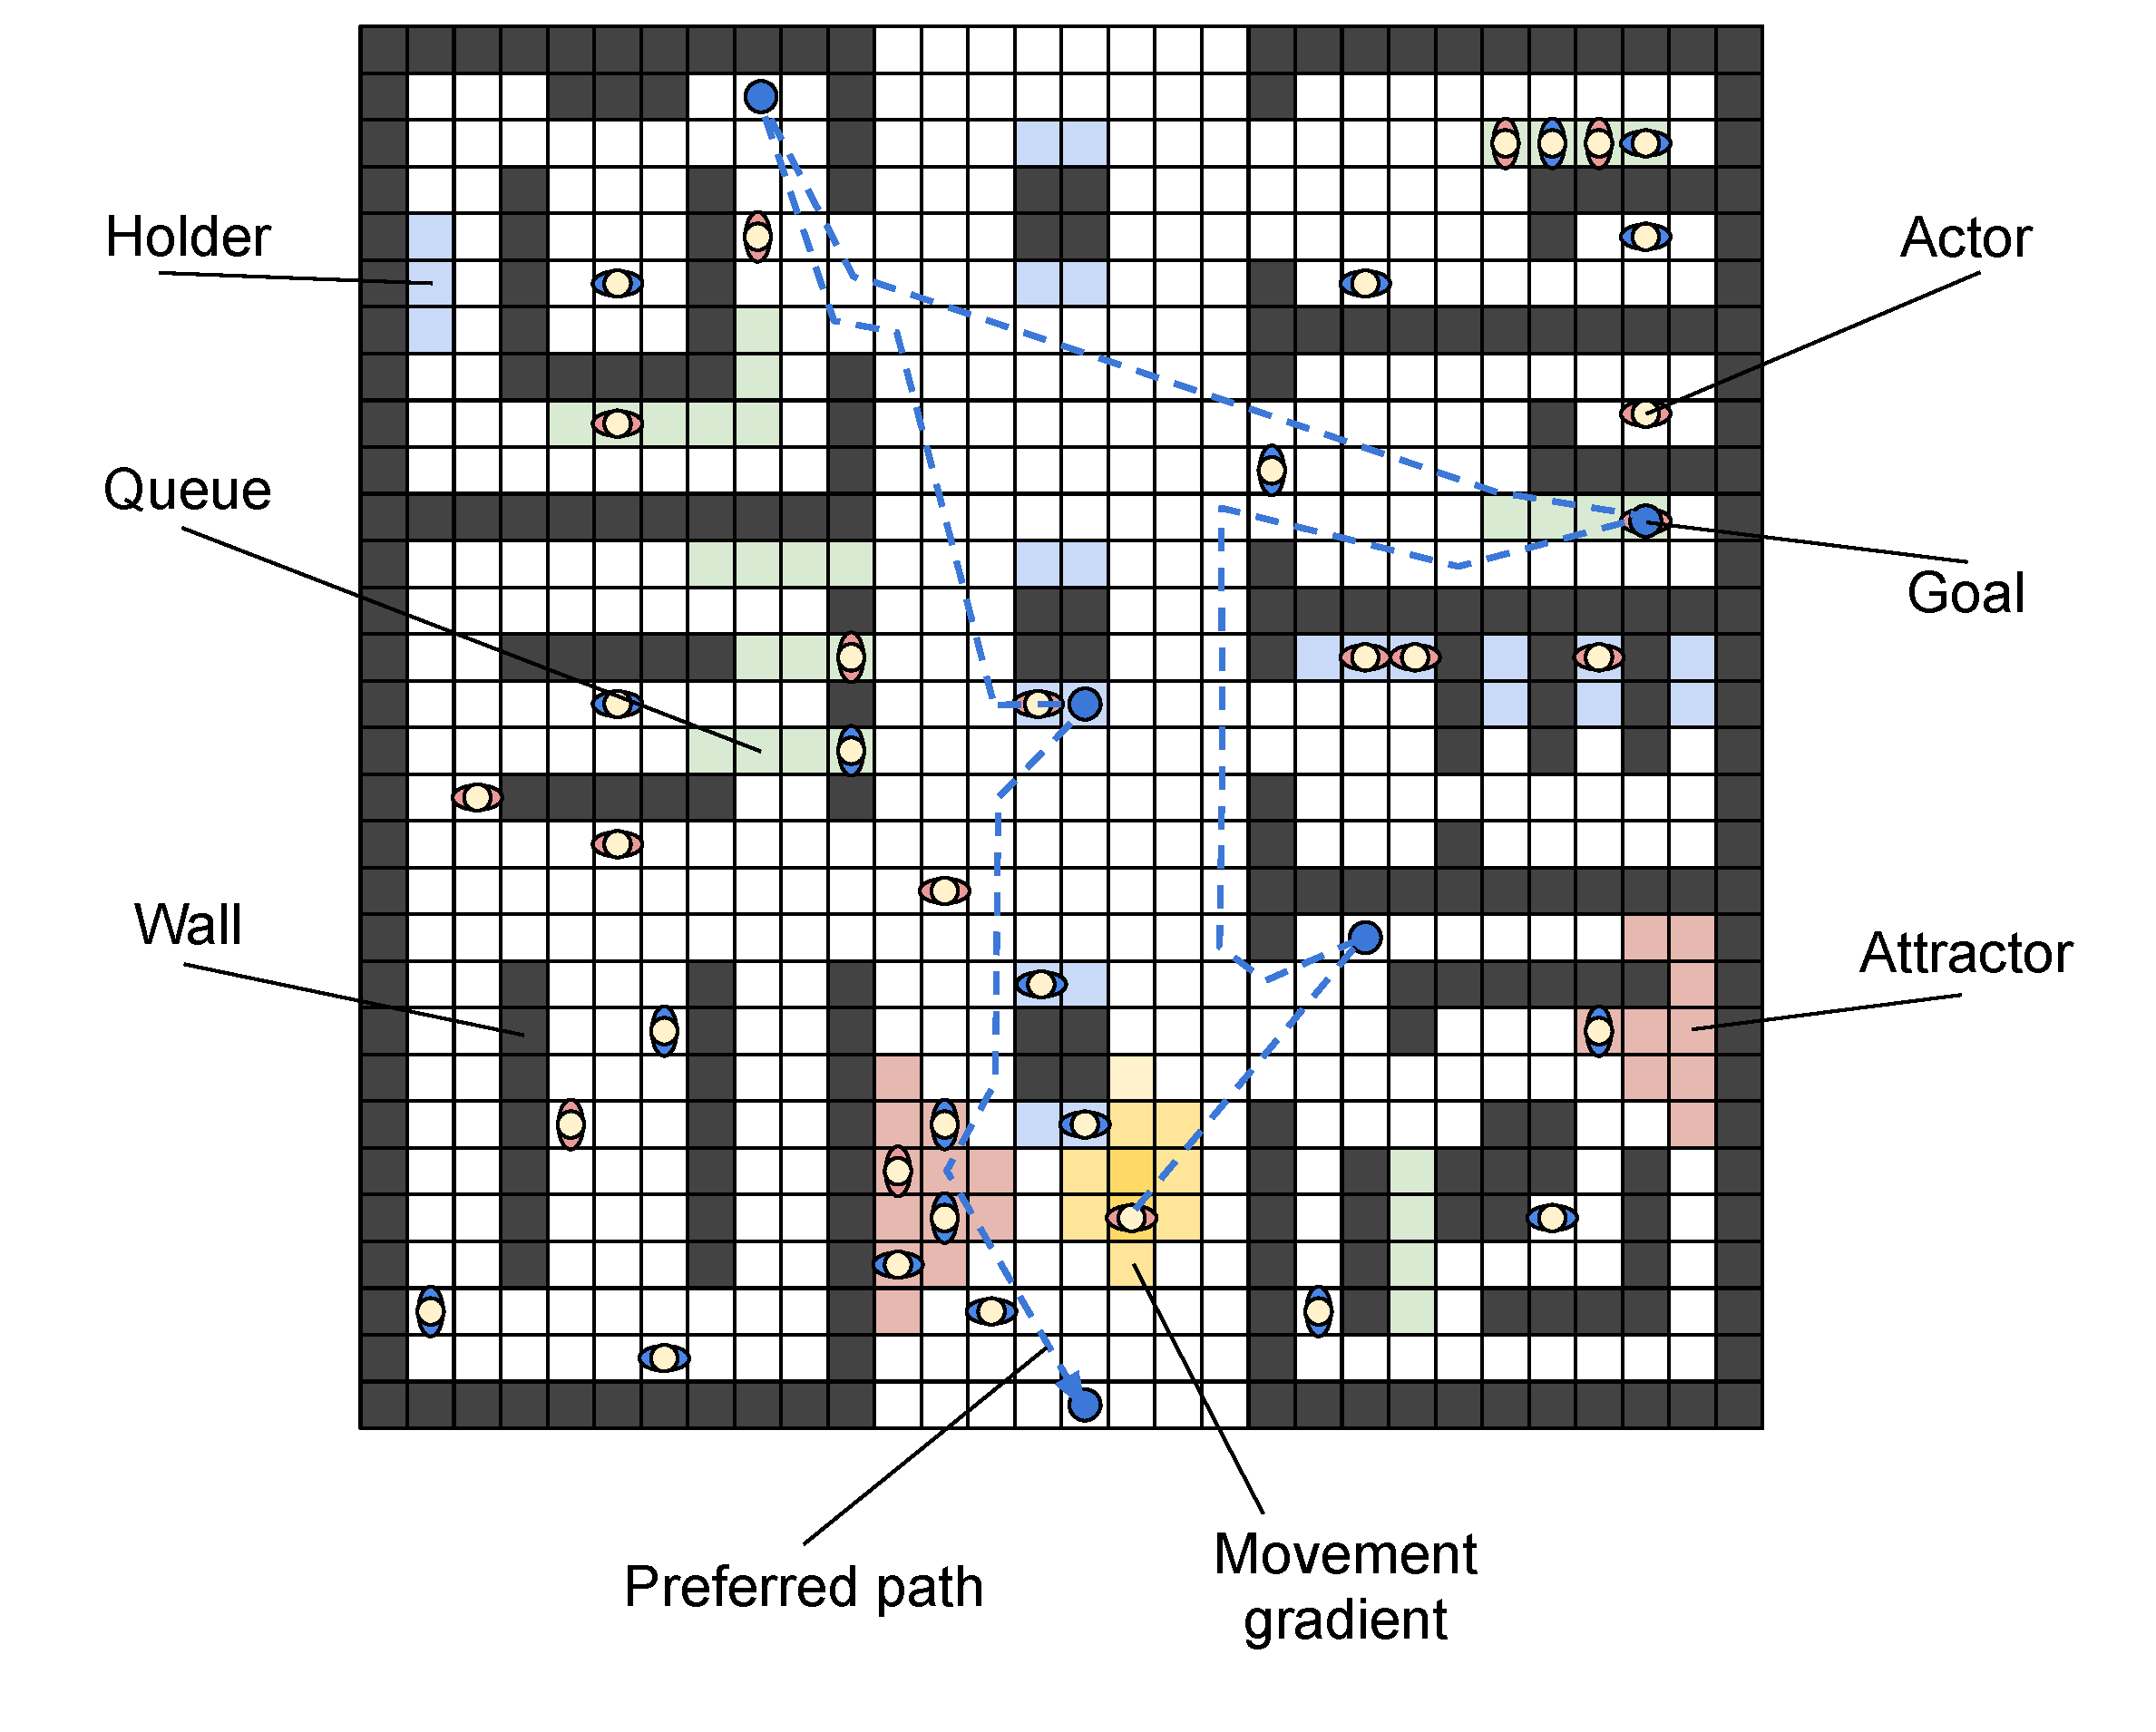
\includegraphics[scale=0.3]{./img/Overview.pdf}
        \caption{Przykładowa dekompozycja problemu.}
        \label{fig:overview}
    \end{figure}

\newpage
    \section{Model ruchu ludzi}
    \label{sec:model}

    \begin{figure}[h!]
        \centering
        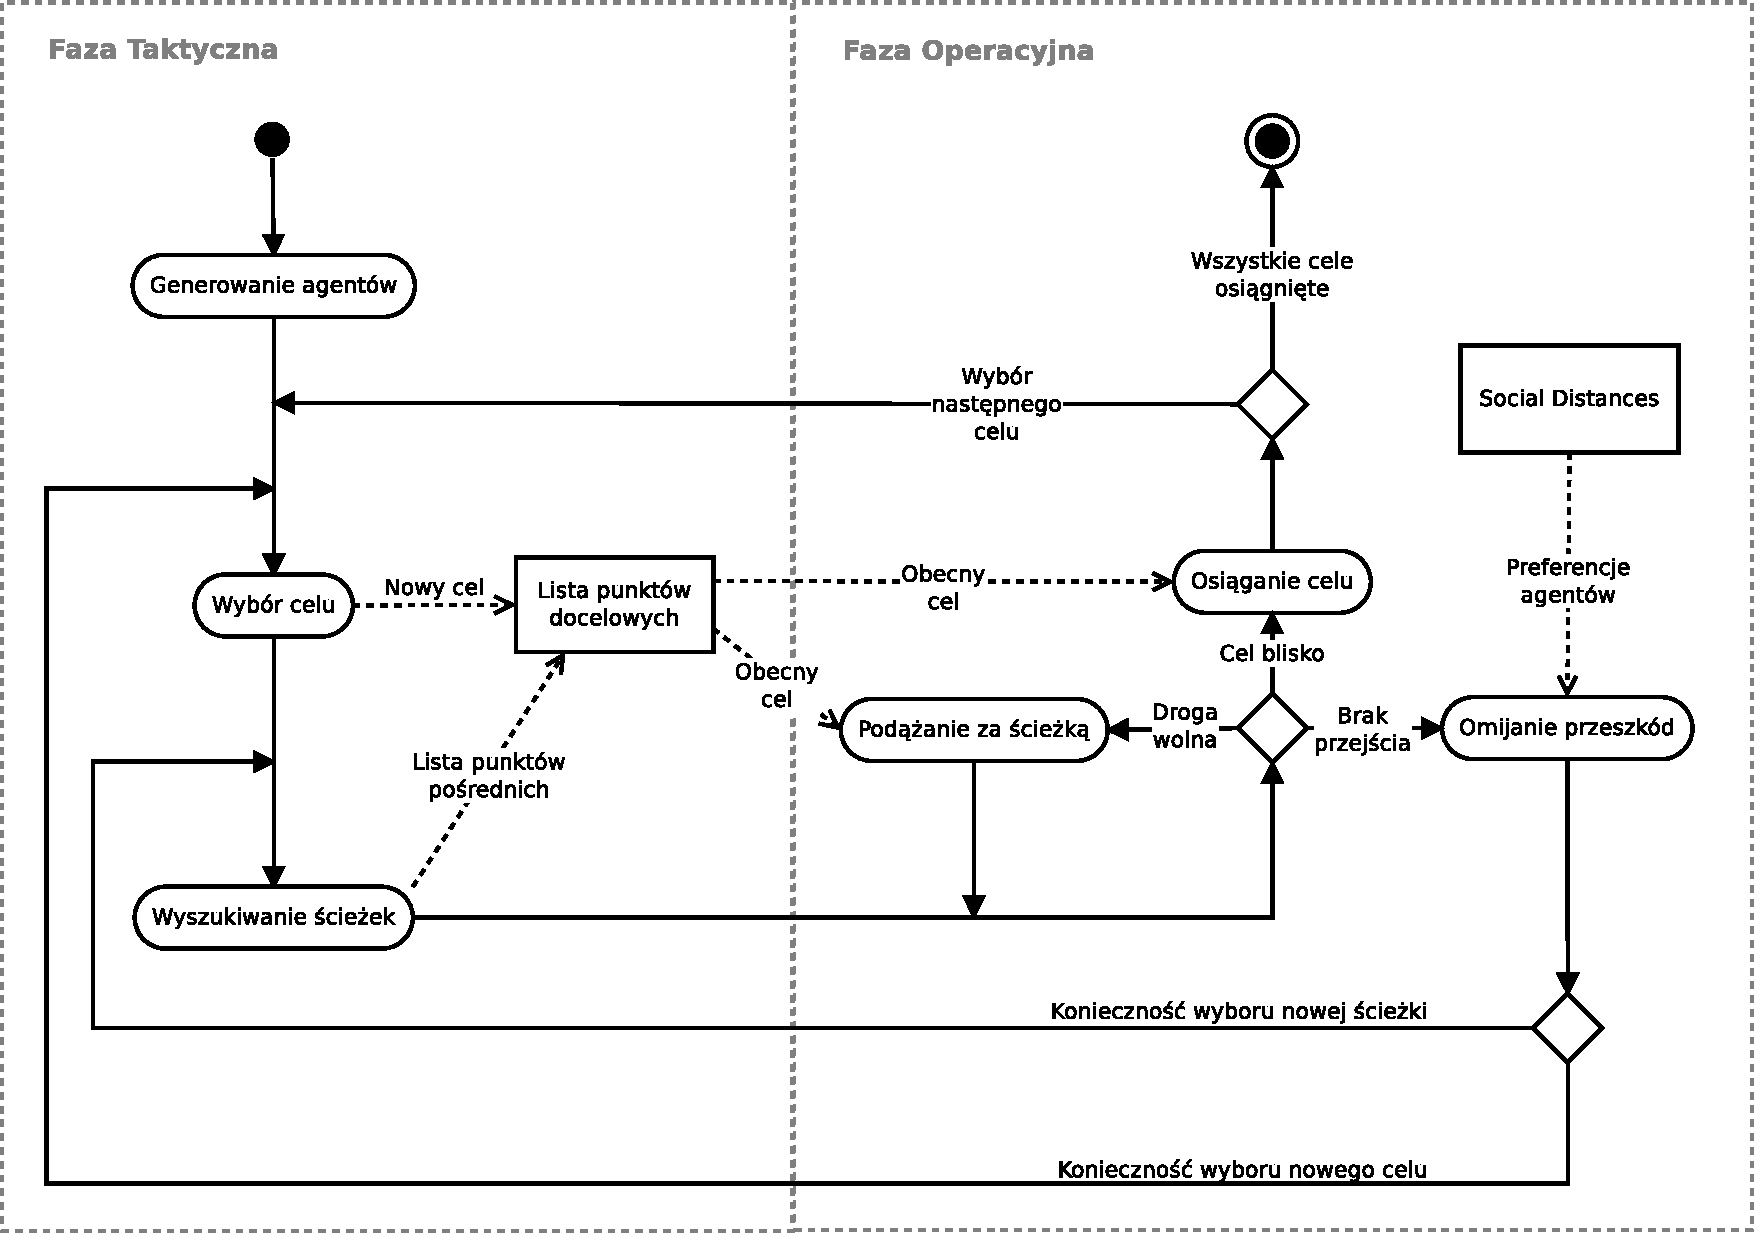
\includegraphics[scale=0.7]{./img/ActorActivity.pdf}
        \caption{Diagram aktywności aktorów.}
        \label{fig:actor-activity}
    \end{figure}


        \subsection{Poziom taktyczny}
        \label{sec:tactical}

        \begin{figure}[h!]
            \centering
            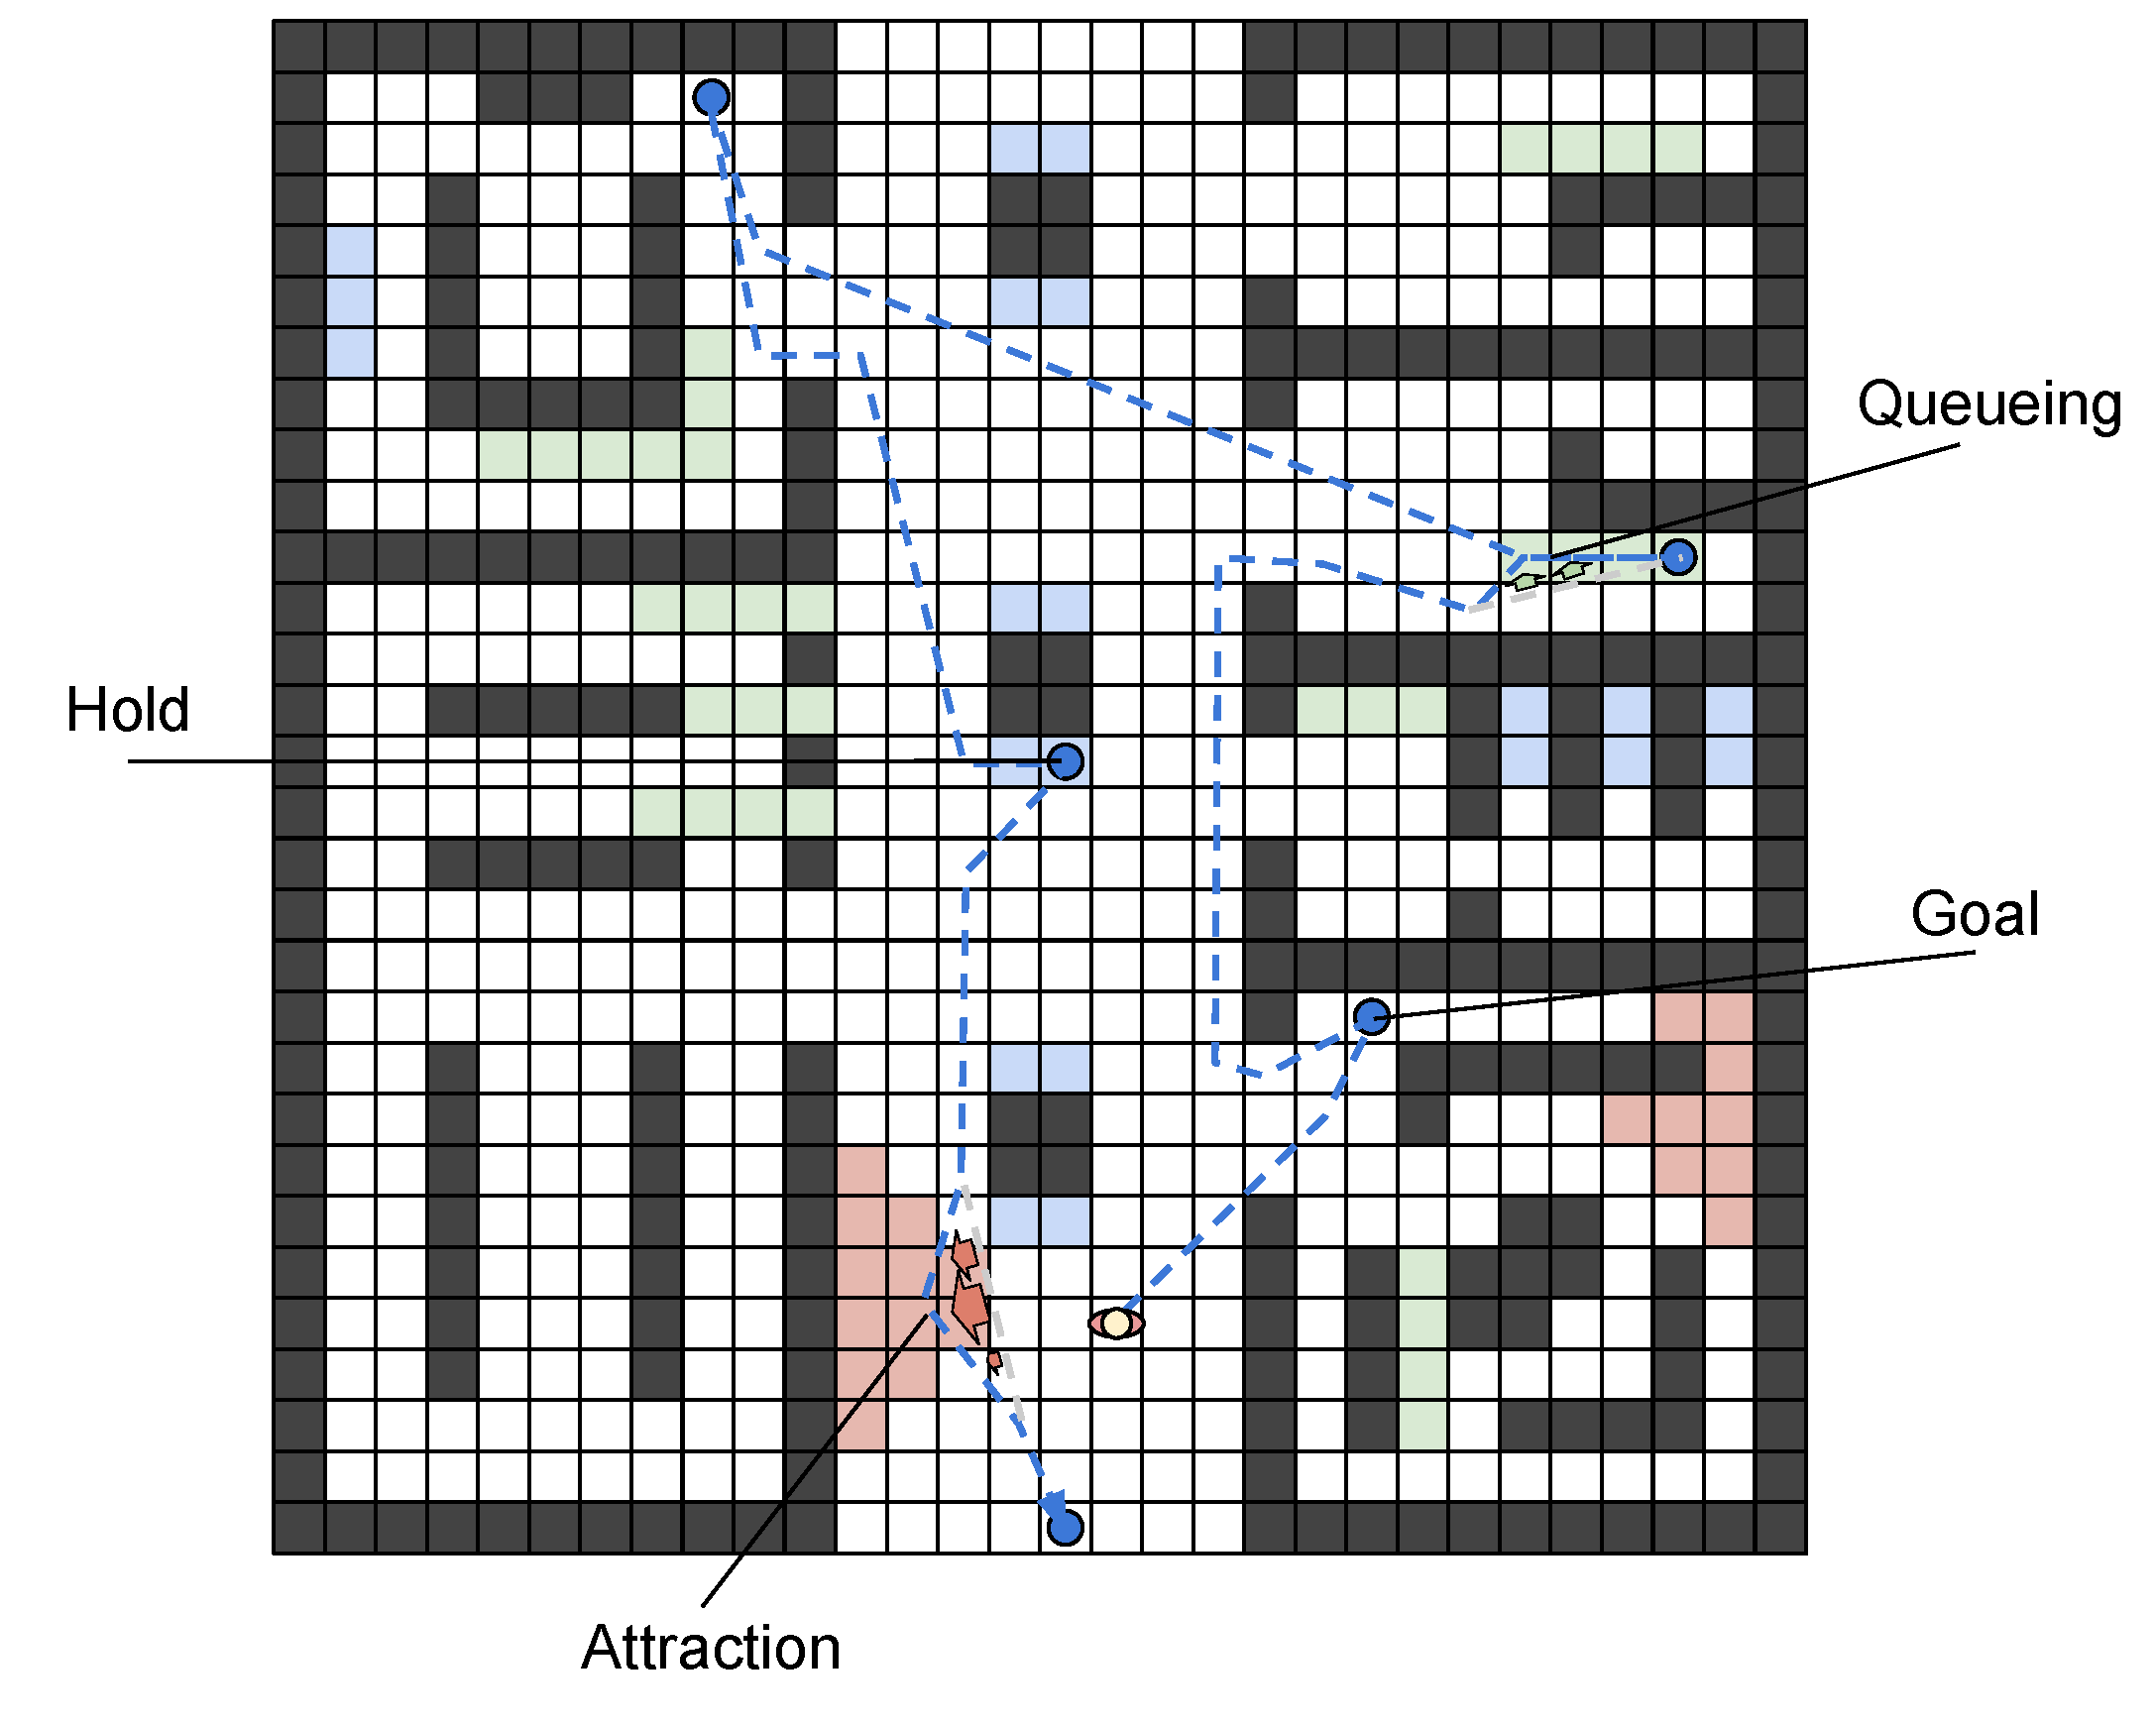
\includegraphics[scale=0.3]{./img/Tactical.pdf}
            \caption{Zakres operacji taktycznej części modelu ruchu.}
            \label{fig:tactical}
        \end{figure}

\noindent
Opis comming soon...

        \subsection{Poziom operacyjny}
        \label{sec:operational}

        \begin{figure}[h!]
            \centering
            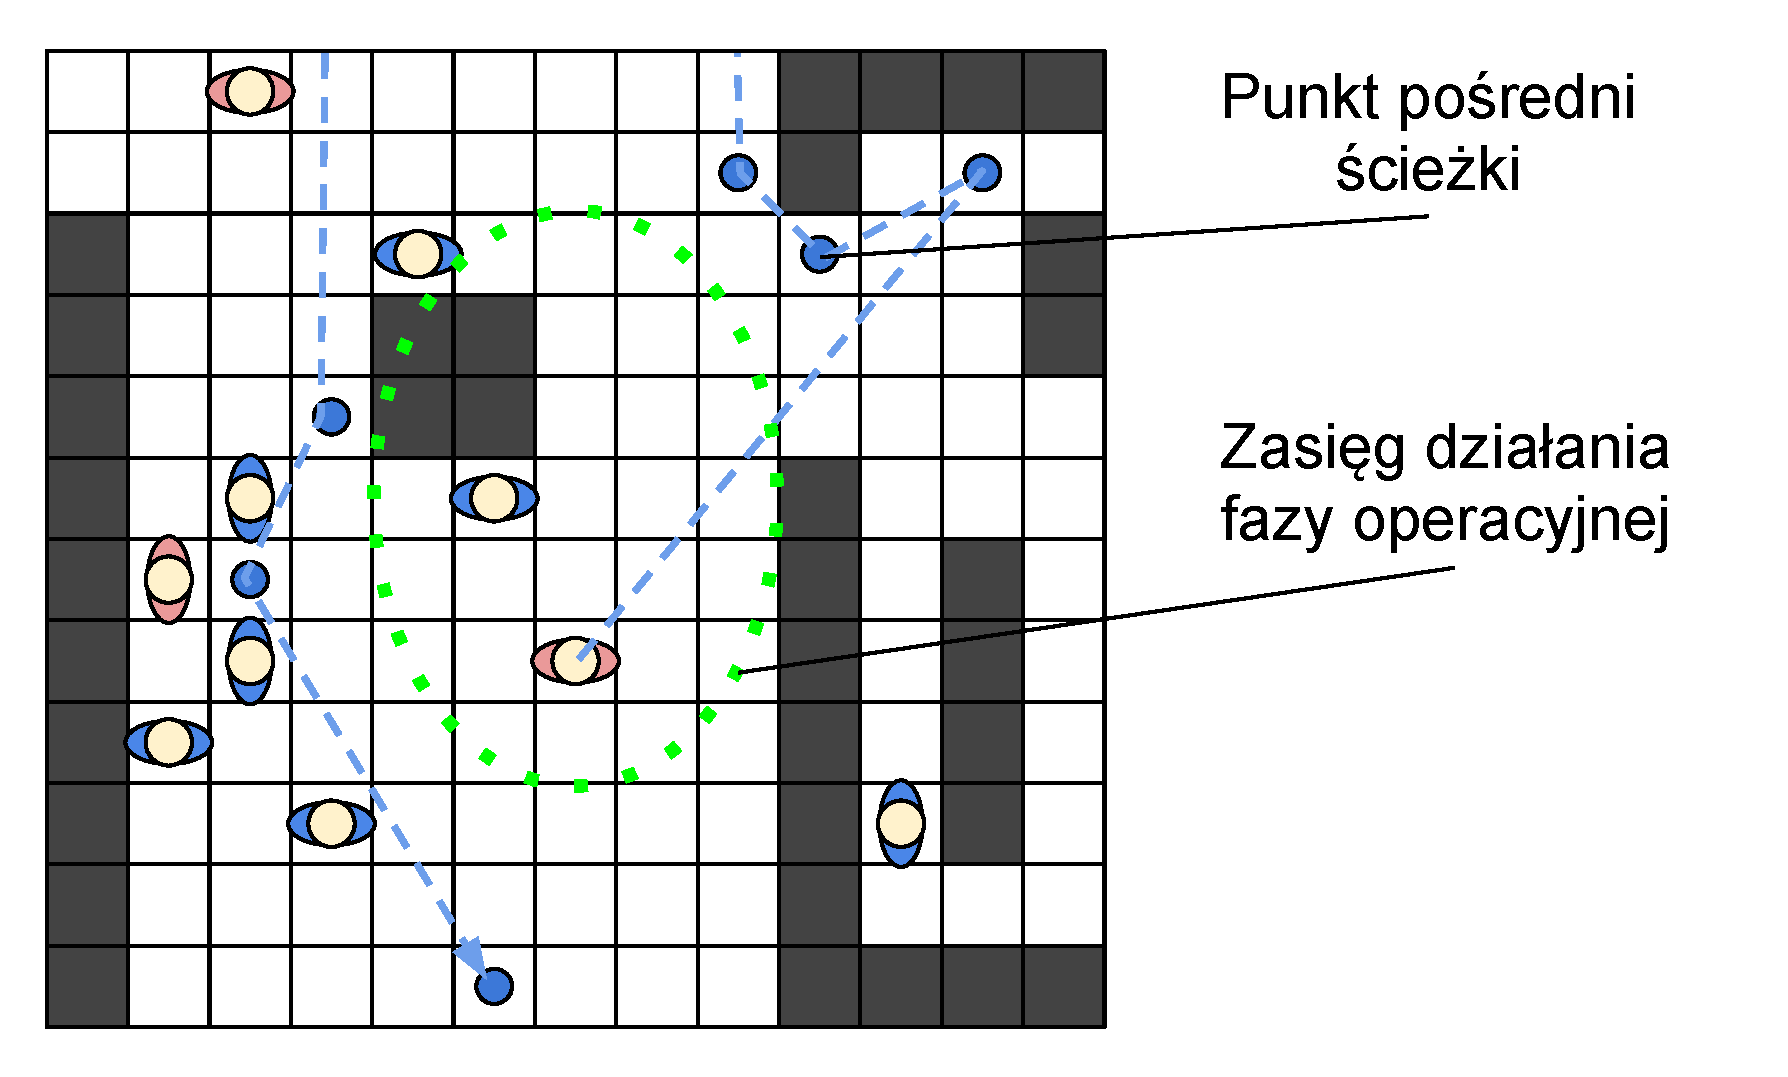
\includegraphics[scale=0.3]{./img/Operative.pdf}
            \caption{Zakres działania operacyjnej części modelu ruchu.}
            \label{fig:operational}
        \end{figure}

\noindent
Opis comming soon...

\newpage
    \section{Implementacja}
    \label{sec:implementation}

        \subsection{Reprezentacja centrum handlowego}
        \label{sec:mall}

        \begin{figure}[h!]
            \centering
            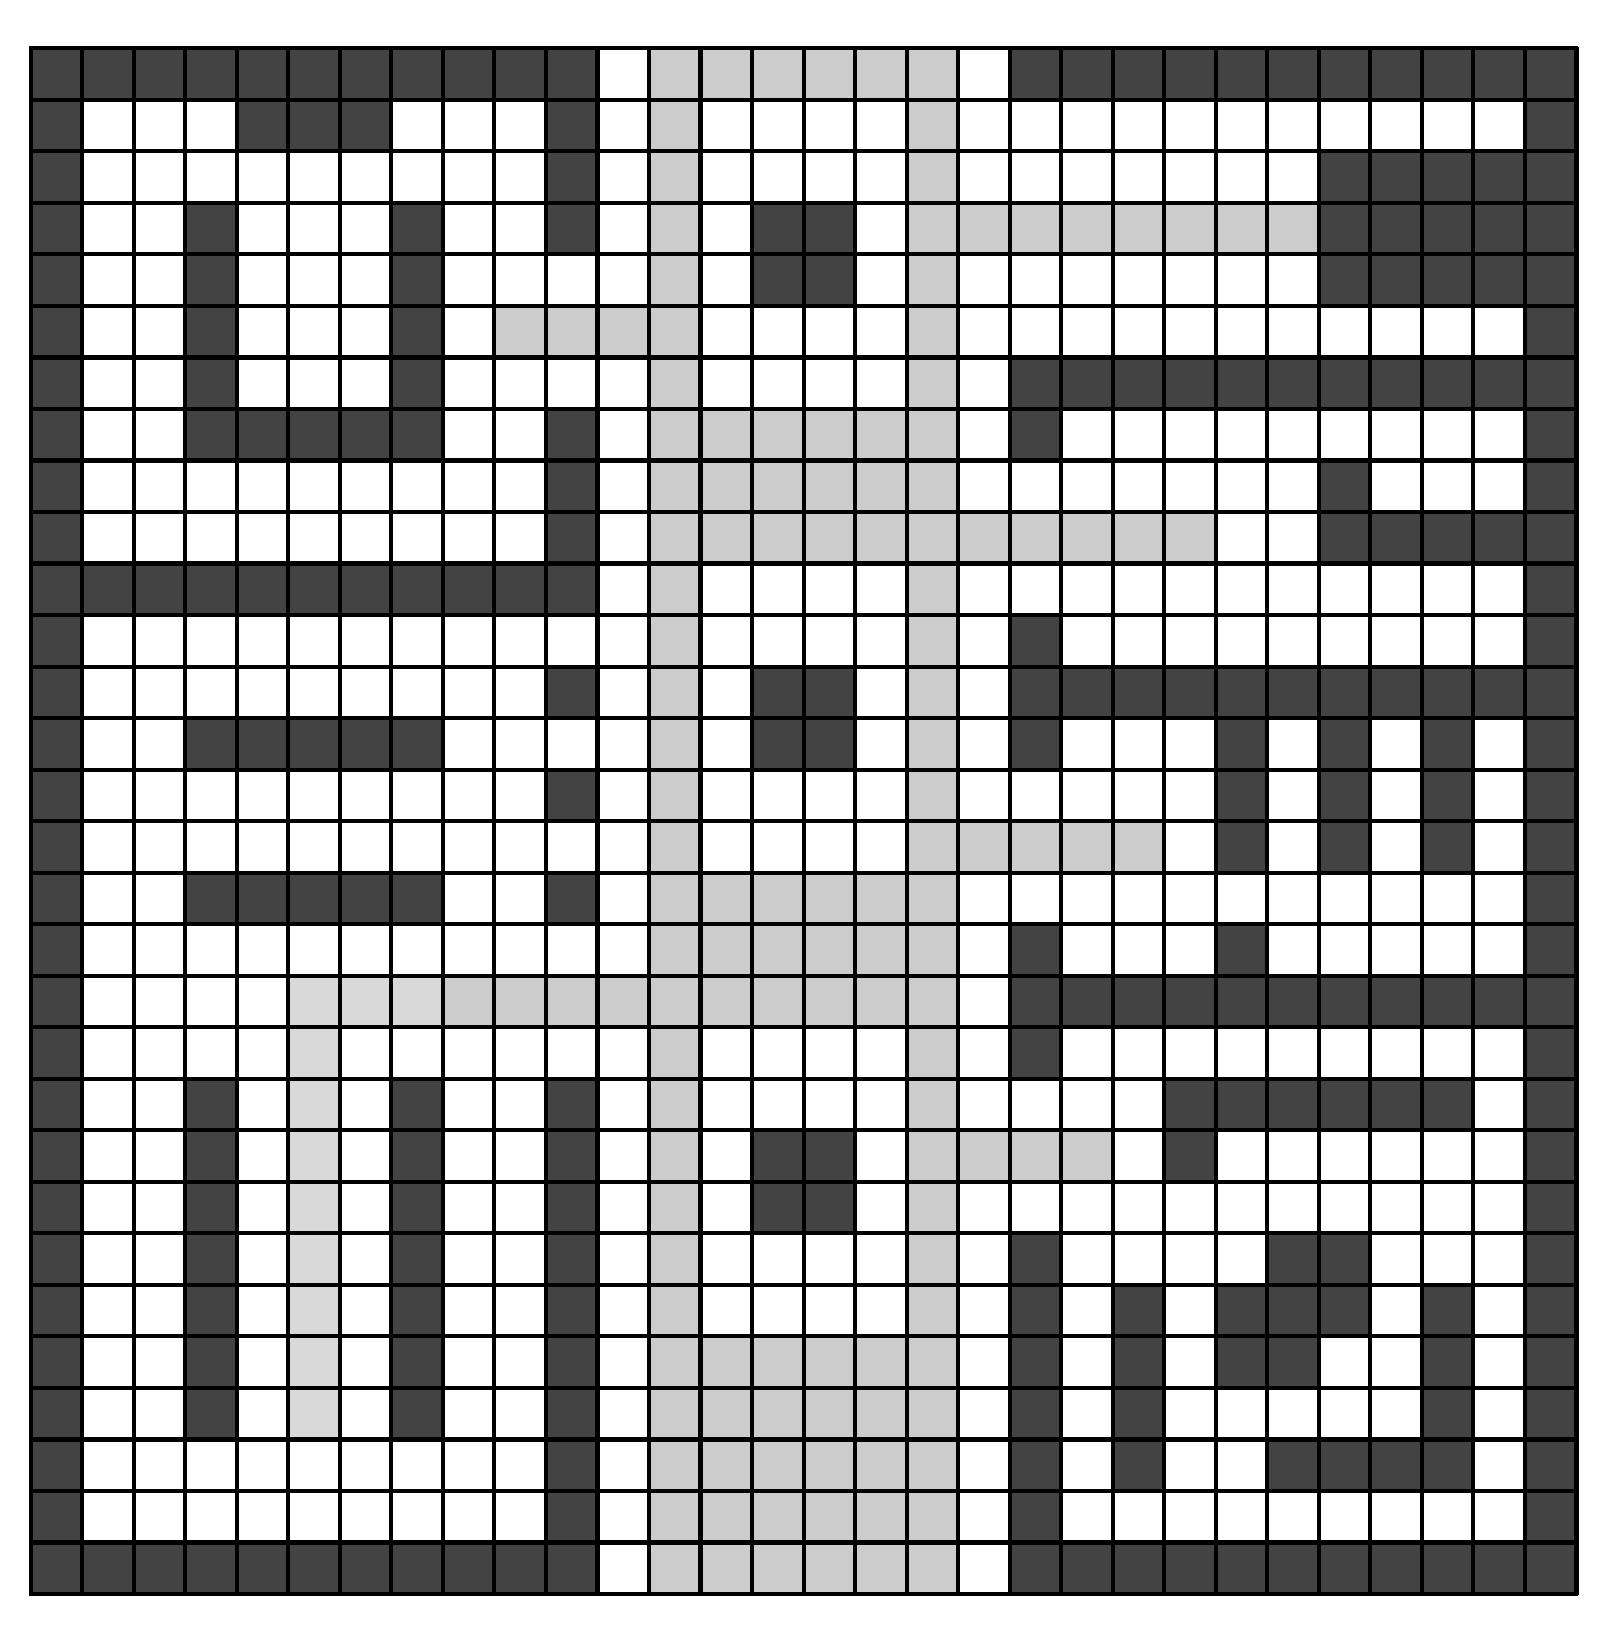
\includegraphics[scale=0.2]{./img/MallLayout.pdf}
            \caption{Przykładowy rozkład pomieszczeń małego centrum handlowego.}
            \label{fig:mall-layout}
        \end{figure}

        \begin{figure}[h!]
            \centering
            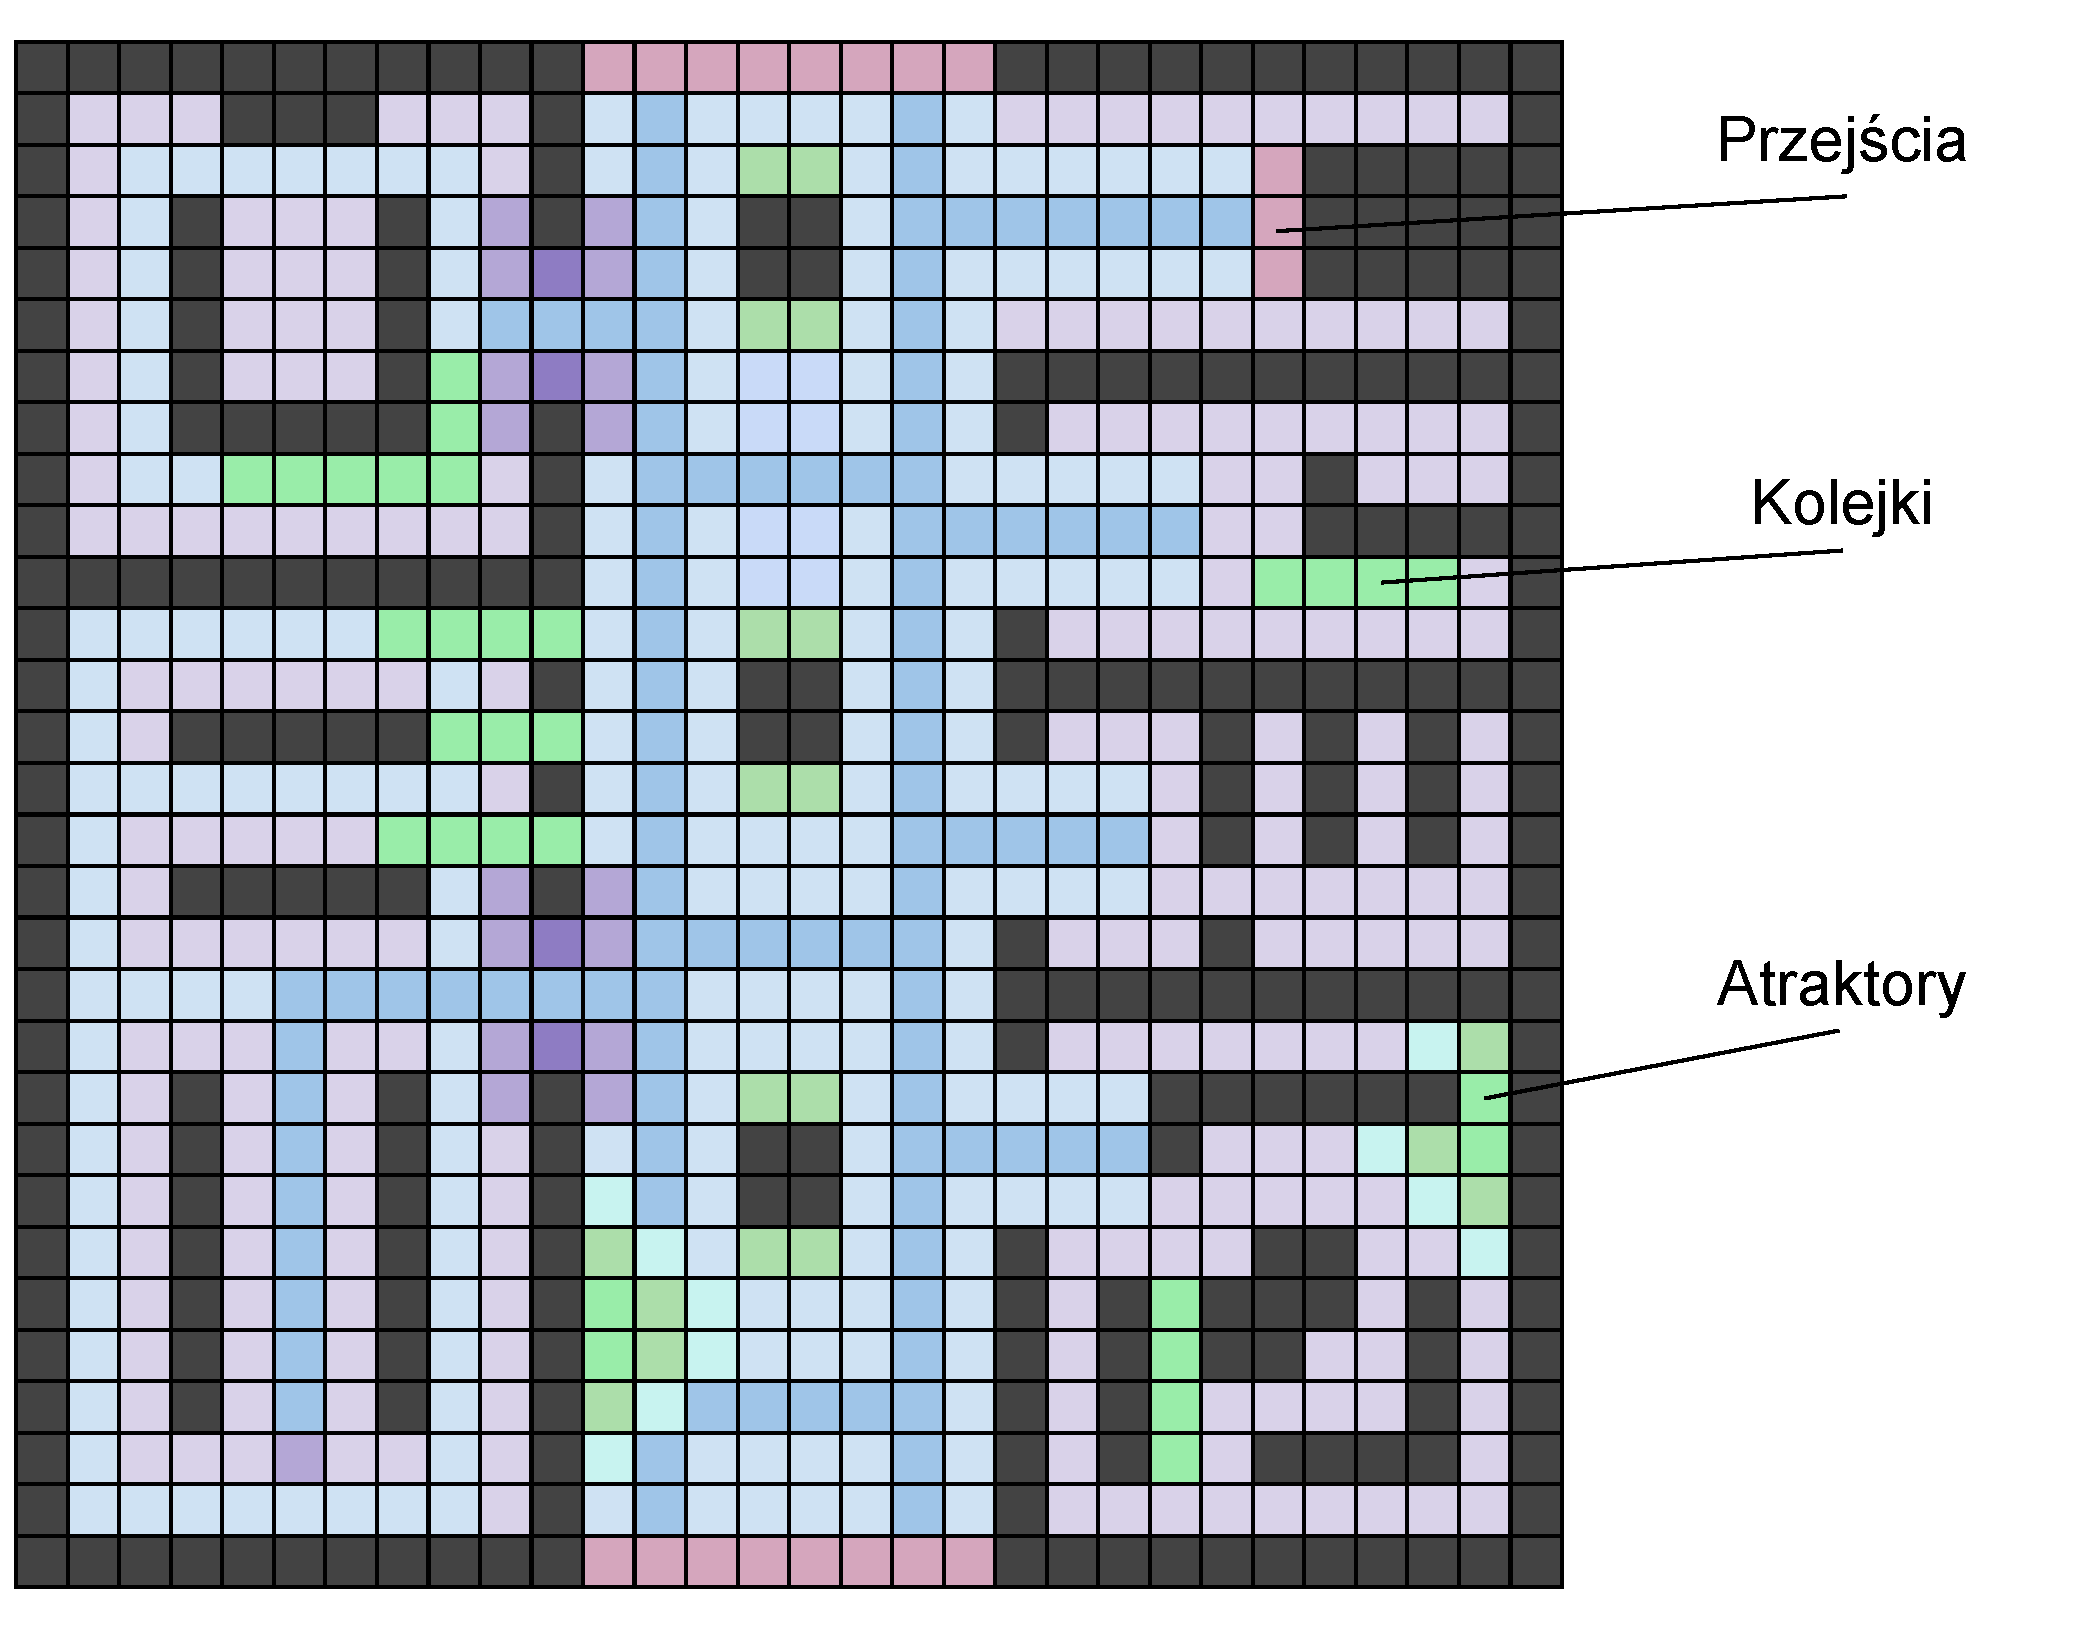
\includegraphics[scale=0.2]{./img/MallFeatures.pdf}
            \caption{Przykładowy rozkład stref specjalnych małego centrum handlowego.}
            \label{fig:mall-features}
        \end{figure}



     %% TODO
\newpage
    \section{Referencje}
    \label{sec:refs}

    \begin{itemize}
        \begin{item} \label{refs:social-distances-1} Social Distances TODO \end{item}
        \item \ldots
    \end{itemize}
    %% TODO
\end{document}
